\documentclass{anstrans}
%%%%%%%%%%%%%%%%%%%%%%%%%%%%%%%%%%%
\title{Hydrogen Economy in Champaign-Urbana}
\author{Roberto E. Fairhurst Agosta, Sammuel Dotson, Kathryn D. Huff}

\institute{
University of Illinois at Urbana-Champaign, Dept. of Nuclear, Plasma, and Radiological Engineering\\
ref3@illinois.edu
}

%%%% packages and definitions (optional)
\usepackage{graphicx} % allows inclusion of graphics
\usepackage{booktabs} % nice rules (thick lines) for tables
\usepackage{microtype} % improves typography for PDF
\usepackage{xspace}
\usepackage{tabularx}
\usepackage{floatrow}
\usepackage{subcaption}
\usepackage{enumitem}
\usepackage{placeins}
\usepackage[acronym,toc]{glossaries}
\newacronym[longplural={metric tons of heavy metal}]{MTHM}{MTHM}{metric ton of heavy metal}
\newacronym{ABM}{ABM}{agent-based modeling}
\newacronym{ACDIS}{ACDIS}{Program in Arms Control \& Domestic and International Security}
\newacronym{AHTR}{AHTR}{Advanced High Temperature Reactor}
\newacronym{ANDRA}{ANDRA}{Agence Nationale pour la gestion des D\'echets RAdioactifs, the French National Agency for Radioactive Waste Management}
\newacronym{APP}{APP}{Abbott Power Plant}
\newacronym{ANL}{ANL}{Argonne National Laboratory}
\newacronym{API}{API}{application programming interface}
\newacronym{ARCH}{ARCH}{autoregressive conditional heteroskedastic}
\newacronym{ARE}{ARE}{Aircraft Reactor Experiment}
\newacronym{ARFC}{ARFC}{Advanced Reactors and Fuel Cycles}
\newacronym{ARMA}{ARMA}{autoregressive moving average}
\newacronym{ASME}{ASME}{American Society of Mechanical Engineers}
\newacronym{ATWS}{ATWS}{Anticipated Transient Without Scram}
\newacronym{BDBE}{BDBE}{Beyond Design Basis Event}
\newacronym{BIDS}{BIDS}{Berkeley Institute for Data Science}
\newacronym{BOL}{BOL}{Beginning-of-Life}
\newacronym{BSD}{BSD}{Berkeley Software Distribution}
\newacronym{CAFCA}{CAFCA}{ Code for Advanced Fuel Cycles Assessment }
\newacronym{CASL}{CASL}{Consortium for Advanced Simulation of Light Water Reactors}
\newacronym{CDTN}{CDTN}{Centro de Desenvolvimento da Tecnologia Nuclear}
\newacronym{CEA}{CEA}{Commissariat \`a l'\'Energie Atomique et aux \'Energies Alternatives}
\newacronym{CI}{CI}{continuous integration}
\newacronym{CNEC}{CNEC}{Consortium for Nonproliferation Enabling Capabilities}
\newacronym{CNEN}{CNEN}{Comiss\~{a}o Nacional de Energia Nuclear}
\newacronym{CNERG}{CNERG}{Computational Nuclear Engineering Research Group}
\newacronym{COSI}{COSI}{Commelini-Sicard}
\newacronym{COTS}{COTS}{commercial, off-the-shelf}
\newacronym{CSNF}{CSNF}{commercial spent nuclear fuel}
\newacronym{CTAH}{CTAHs}{Coiled Tube Air Heaters}
\newacronym{CUBIT}{CUBIT}{CUBIT Geometry and Mesh Generation Toolkit}
\newacronym{CURIE}{CURIE}{Centralized Used Fuel Resource for Information Exchange}
\newacronym{DAG}{DAG}{directed acyclic graph}
\newacronym{DANESS}{DANESS}{Dynamic Analysis of Nuclear Energy System Strategies}
\newacronym{DBE}{DBE}{Design Basis Event}
\newacronym{DESAE}{DESAE}{Dynamic Analysis of Nuclear Energy Systems Strategies}
\newacronym{DHS}{DHS}{Department of Homeland Security}
\newacronym{DOE}{DOE}{Department of Energy}
\newacronym{DRACS}{DRACS}{Direct Reactor Auxiliary Cooling System}
\newacronym{DRE}{DRE}{dynamic resource exchange}
\newacronym{DSNF}{DSNF}{DOE spent nuclear fuel}
\newacronym{DYMOND}{DYMOND}{Dynamic Model of Nuclear Development }
\newacronym{EBS}{EBS}{Engineered Barrier System}
\newacronym{EDZ}{EDZ}{Excavation Disturbed Zone}
\newacronym{EIA}{EIA}{U.S. Energy Information Administration}
\newacronym{EPA}{EPA}{Environmental Protection Agency}
\newacronym{EP}{EP}{Engineering Physics}
\newacronym{FCO}{FCO}{Fuel Cycle Options}
\newacronym{FCT}{FCT}{Fuel Cycle Technology}
\newacronym{FCWMD}{FCWMD}{Fuel Cycle and Waste Management Division}
\newacronym{FEHM}{FEHM}{Finite Element Heat and Mass Transfer}
\newacronym{FEPs}{FEPs}{Features, Events, and Processes}
\newacronym{FHR}{FHR}{Fluoride-Salt-Cooled High-Temperature Reactor}
\newacronym{FLiBe}{FLiBe}{Fluoride-Lithium-Beryllium}
\newacronym{GCAM}{GCAM}{Global Change Assessment Model}
\newacronym{GDSE}{GDSE}{Generic Disposal System Environment}
\newacronym{GDSM}{GDSM}{Generic Disposal System Model}
\newacronym{GENIUSv1}{GENIUSv1}{Global Evaluation of Nuclear Infrastructure Utilization Scenarios, Version 1}
\newacronym{GENIUSv2}{GENIUSv2}{Global Evaluation of Nuclear Infrastructure Utilization Scenarios, Version 2}
\newacronym{GENIUS}{GENIUS}{Global Evaluation of Nuclear Infrastructure Utilization Scenarios}
\newacronym{GPAM}{GPAM}{Generic Performance Assessment Model}
\newacronym{GRSAC}{GRSAC}{Graphite Reactor Severe Accident Code}
\newacronym{GUI}{GUI}{graphical user interface}
\newacronym{HLW}{HLW}{high level waste}
\newacronym{HPC}{HPC}{high-performance computing}
\newacronym{HTC}{HTC}{high-throughput computing}
\newacronym{HTGR}{HTGR}{High Temperature Gas-Cooled Reactor}
\newacronym{IAEA}{IAEA}{International Atomic Energy Agency}
\newacronym{IEMA}{IEMA}{Illinois Emergency Mangament Agency}
\newacronym{INL}{INL}{Idaho National Laboratory}
\newacronym{IPRR1}{IRP-R1}{Instituto de Pesquisas Radioativas Reator 1}
\newacronym{IRP}{IRP}{Integrated Research Project}
\newacronym{ISFSI}{ISFSI}{Independent Spent Fuel Storage Installation}
\newacronym{ISRG}{ISRG}{Independent Student Research Group}
\newacronym{JFNK}{JFNK}{Jacobian-Free Newton Krylov}
\newacronym{LANL}{LANL}{Los Alamos National Laboratory}
\newacronym{LBNL}{LBNL}{Lawrence Berkeley National Laboratory}
\newacronym{LCOE}{LCOE}{levelized cost of electricity}
\newacronym{LDRD}{LDRD}{laboratory directed research and development}
\newacronym{LFR}{LFR}{Lead-Cooled Fast Reactor}
\newacronym{LGPL}{LGPL}{Lesser GNU Public License}
\newacronym{LLNL}{LLNL}{Lawrence Livermore National Laboratory}
\newacronym{LMFBR}{LMFBR}{Liquid-Metal-cooled Fast Breeder Reactor}
\newacronym{LOFC}{LOFC}{Loss of Forced Cooling}
\newacronym{LOHS}{LOHS}{Loss of Heat Sink}
\newacronym{LOLA}{LOLA}{Loss of Large Area}
\newacronym{LP}{LP}{linear program}
\newacronym{LWR}{LWR}{Light Water Reactor}
\newacronym{MARKAL}{MARKAL}{MARKet and ALlocation}
\newacronym{MA}{MA}{minor actinide}
\newacronym{MCNP}{MCNP}{Monte Carlo N-Particle code}
\newacronym{MILP}{MILP}{mixed-integer linear program}
\newacronym{MIT}{MIT}{the Massachusetts Institute of Technology}
\newacronym{MOAB}{MOAB}{Mesh-Oriented datABase}
\newacronym{MOOSE}{MOOSE}{Multiphysics Object-Oriented Simulation Environment}
\newacronym{MOX}{MOX}{mixed oxide}
\newacronym{MSBR}{MSBR}{Molten Salt Breeder Reactor}
\newacronym{MSRE}{MSRE}{Molten Salt Reactor Experiment}
\newacronym{MSR}{MSR}{Molten Salt Reactor}
\newacronym{NAGRA}{NAGRA}{National Cooperative for the Disposal of Radioactive Waste}
\newacronym{NCSA}{NCSA}{National Center for Supercomputing Applications}
\newacronym{NEAMS}{NEAMS}{Nuclear Engineering Advanced Modeling and Simulation}
\newacronym{NEUP}{NEUP}{Nuclear Energy University Programs}
\newacronym{NFCSim}{NFCSim}{Nuclear Fuel Cycle Simulator}
\newacronym{NFC}{NFC}{Nuclear Fuel Cycle}
\newacronym{NGNP}{NGNP}{Next Generation Nuclear Plant}
\newacronym{NMWPC}{NMWPC}{Nuclear MW Per Capita}
\newacronym{NNSA}{NNSA}{National Nuclear Security Administration}
\newacronym{NPRE}{NPRE}{Department of Nuclear, Plasma, and Radiological Engineering}
\newacronym{NQA1}{NQA-1}{Nuclear Quality Assurance - 1}
\newacronym{NRC}{NRC}{Nuclear Regulatory Commission}
\newacronym{NSF}{NSF}{National Science Foundation}
\newacronym{NSSC}{NSSC}{Nuclear Science and Security Consortium}
\newacronym{NUWASTE}{NUWASTE}{Nuclear Waste Assessment System for Technical Evaluation}
\newacronym{NWF}{NWF}{Nuclear Waste Fund}
\newacronym{NWTRB}{NWTRB}{Nuclear Waste Technical Review Board}
\newacronym{OCRWM}{OCRWM}{Office of Civilian Radioactive Waste Management}
\newacronym{ORION}{ORION}{ORION}
\newacronym{ORNL}{ORNL}{Oak Ridge National Laboratory}
\newacronym{PARCS}{PARCS}{Purdue Advanced Reactor Core Simulator}
\newacronym{PBAHTR}{PB-AHTR}{Pebble Bed Advanced High Temperature Reactor}
\newacronym{PBFHR}{PB-FHR}{Pebble-Bed Fluoride-Salt-Cooled High-Temperature Reactor}
\newacronym{PEI}{PEI}{Peak Environmental Impact}
\newacronym{PH}{PRONGHORN}{PRONGHORN}
\newacronym{PI}{PI}{Principal Investigator}
\newacronym{PNNL}{PNNL}{Pacific Northwest National Laboratory}
\newacronym{PRIS}{PRIS}{Power Reactor Information System}
\newacronym{PRKE}{PRKE}{Point Reactor Kinetics Equations}
\newacronym{PSPG}{PSPG}{Pressure-Stabilizing/Petrov-Galerkin}
\newacronym{PWAR}{PWAR}{Pratt and Whitney Aircraft Reactor}
\newacronym{PWR}{PWR}{Pressurized Water Reactor}
\newacronym{PyNE}{PyNE}{Python toolkit for Nuclear Engineering}
\newacronym{PyRK}{PyRK}{Python for Reactor Kinetics}
\newacronym{QA}{QA}{quality assurance}
\newacronym{RDD}{RD\&D}{Research Development and Demonstration}
\newacronym{RD}{R\&D}{Research and Development}
\newacronym{RELAP}{RELAP}{Reactor Excursion and Leak Analysis Program}
\newacronym{RIA}{RIA}{Reactivity Insertion Accident}
\newacronym{RIF}{RIF}{Region-Institution-Facility}
\newacronym{SAM}{SAM}{Simulation and Modeling}
\newacronym{SCF}{SCF}{Software Carpentry Foundation}
\newacronym{SFR}{SFR}{Sodium-Cooled Fast Reactor}
\newacronym{SINDAG}{SINDA{\textbackslash}G}{Systems Improved Numerical Differencing Analyzer $\backslash$ Gaski}
\newacronym{SKB}{SKB}{Svensk K\"{a}rnbr\"{a}nslehantering AB}
\newacronym{SNF}{SNF}{spent nuclear fuel}
\newacronym{SNL}{SNL}{Sandia National Laboratory}
\newacronym{SNM}{SNM}{Special Nuclear Material}
\newacronym{STC}{STC}{specific temperature change}
\newacronym{SUPG}{SUPG}{Streamline-Upwind/Petrov-Galerkin}
\newacronym{SWF}{SWF}{Separations and Waste Forms}
\newacronym{SWU}{SWU}{Separative Work Unit}
\newacronym{SandO}{S\&O}{Signatures and Observables}
\newacronym{THW}{THW}{The Hacker Within}
\newacronym{TRIGA}{TRIGA}{Training Research Isotope General Atomic}
\newacronym{TRISO}{TRISO}{Tristructural Isotropic}
\newacronym{TSM}{TSM}{Total System Model}
\newacronym{TSPA}{TSPA}{Total System Performance Assessment for the Yucca Mountain License Application}
\newacronym{UDB}{UDB}{Unified Database}
\newacronym{UFD}{UFD}{Used Fuel Disposition}
\newacronym{UML}{UML}{Unified Modeling Language}
\newacronym{UNFSTANDARDS}{UNFST\&DARDS}{Used Nuclear Fuel Storage, Transportation \& Disposal Analysis Resource and Data System}
\newacronym{UOX}{UOX}{uranium oxide}
\newacronym{UQ}{UQ}{uncertainty quantification}
\newacronym{US}{US}{United States}
\newacronym{UW}{UW}{University of Wisconsin}
\newacronym{VISION}{VISION}{the Verifiable Fuel Cycle Simulation Model}
\newacronym{VV}{V\&V}{verification and validation}
\newacronym{WIPP}{WIPP}{Waste Isolation Pilot Plant}
\newacronym{YMG}{YMG}{Young Members Group}
\newacronym{YMR}{YMR}{Yucca Mountain Repository Site}
\newacronym{NEI}{NEI}{Nuclear Energy Institute}
%\newacronym{<++>}{<++>}{<++>}
%\newacronym{<++>}{<++>}{<++>}

\makeglossaries

\newcommand{\SN}{S$_N$}
\renewcommand{\vec}[1]{\bm{#1}} %vector is bold italic
\newcommand{\vd}{\bm{\cdot}} % slightly bold vector dot
\newcommand{\grad}{\vec{\nabla}} % gradient
\newcommand{\ud}{\mathop{}\!\mathrm{d}} % upright derivative symbol

\newcolumntype{c}{>{\hsize=.56\hsize}X}
\newcolumntype{b}{>{\hsize=.7\hsize}X}
\newcolumntype{s}{>{\hsize=.74\hsize}X}
\newcolumntype{f}{>{\hsize=.1\hsize}X}
\newcolumntype{a}{>{\hsize=.45\hsize}X}
\usepackage{titlesec}
\titleformat*{\subsection}{\normalfont}

\begin{document}
%%%%%%%%%%%%%%%%%%%%%%%%%%%%%%%%%%%%%%%%%%%%%%%%%%%%%%%%%%%%%%%%%%%%%%%%%%%%%%%%
\section{Introduction}

The Illinois Climate Action Plan (iCAP) focuses on making UIUC campus more sustainable. One of the objectives listed in the iCAP is the reduction of carbon emissions. As Figure \ref{fig:ghg} displays, transportation was the economic sector that produced the largest amount of greenhouse emissions in the US in 2017. It is important to decarbonize transportation on UIUC campus in order to reach the iCAP goal and halt climate change \cite{noauthor_illlinois_2015}.

\begin{figure}[H]
	\centering
	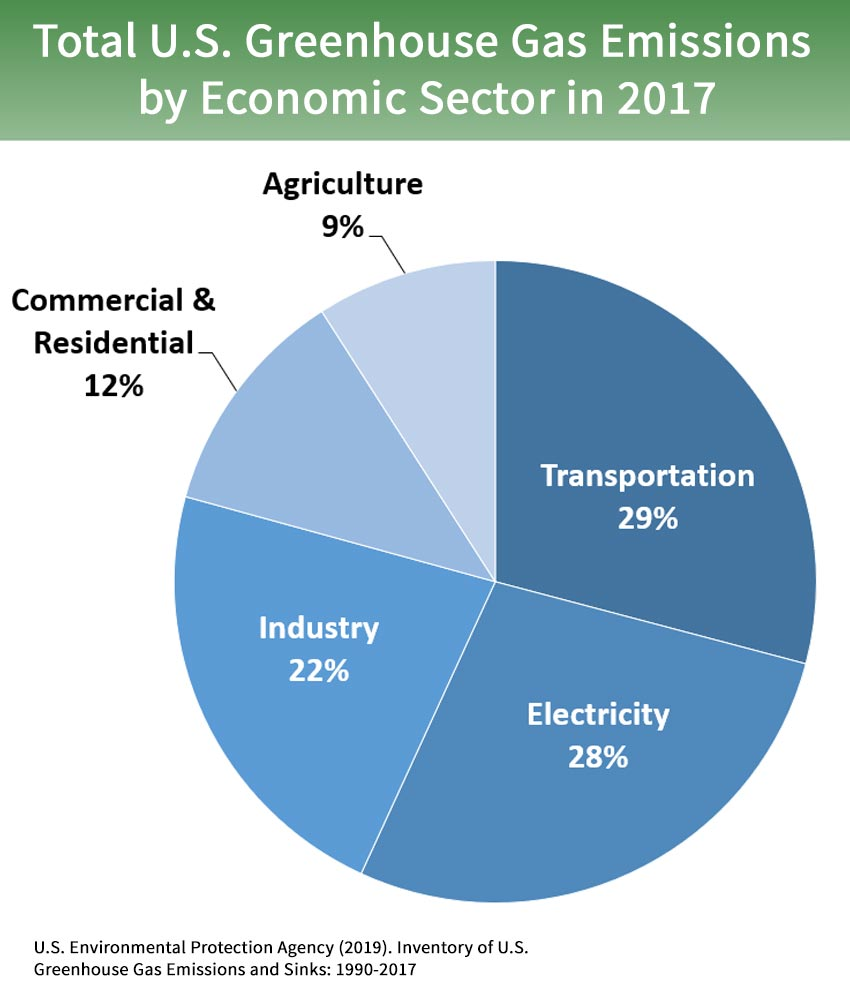
\includegraphics[width=0.5\linewidth]{figures/total-ghg-2019-caption.jpg}
	\hfill
	\caption{Total U.S. Greenhouse Gas Emissions by Economic Sector in 2017 \cite{us_epa_sources_2020}.}
	\label{fig:ghg}
\end{figure}

One possible solution to reduce carbon emissions, and even achieve a net zero carbon production, is to develop hydrogen economies as California is currently doing \cite{brown_economic_2013}. This article presents a few hydrogen production methods. As Section \ref{hydroprod} will describe in the following, some of the methods presented here help reduce carbon emissions but do not eliminate the production of CO$_2$. Nuclear reactors introduce a solution to this problem by producing clean H$_2$ and heat for use in other industrial processes.

Micro-Reactors are an innovative technology that is very attractive for hydrogen production. This type of reactors has three main features: Factory fabricated, transportable, and self-regulating. All the components fully assembled in a factory and shipped out to location will reduce capital costs and allow to deploy the reactor quickly. Simple design concepts will eliminate the need of a large number of specialized operators. They will utilize passive safey systems that prevent overheating or meltdown \cite{noauthor_ultimate_2019}.

Section \ref{method} explains the method used to calculate the amount of hydrogen required to fuel UIUC campus fleet service vehicles and Champaign-Urbana Mass Transit District (MTD) bus system.

\section{Hydrogen Production Methods}
\label{hydroprod}

Some hydrogen production processes are: 
\begin{description}[font=$\bullet$\scshape\bfseries]
	\item[] Steam-Methane Reforming (aka Natural Gas Reforming).
	\item[] Electrolysis.
	\item[] High-Temperature Electrolysis.
	\item[] Iodine-Sulfur Thermochemical Cycle.
	\item[] Coal Gasification with CCS (aka Carbon Sequestration).
	\item[] Solar Thermochemical Hydrogen Production.
\end{description}

The two most common methods for producing hydrogen are steam reforming and electrolysis.

\subsection{Steam Reforming}

Steam reforming is currently the least expensive way to produce hydrogen. This method separates hydrogen atoms from carbon atoms in methane (CH4). This process results in carbon dioxide emissions.
Steam reforming is a mature production process that uses high-temperature steam (700$^{\circ}$C-1000$^{\circ}$C) to produce hydrogen from a methane source. Methane reacts with steam under 3-25 bar pressure in the presence of a catalyst to produce hydrogen, carbon monoxide, and a small portion of carbon dioxide. The reaction is endothermic and requires the supply of heat to occur \cite{noauthor_hydrogen_nodate}:
\begin{equation}
CH_4 + H_2O + heat \rightarrow CO + 3H_2
\end{equation}
A secondary reaction known as water-gas shift reaction occurs producing $CO_2$ and more hydrogen:
\begin{equation}
CO + H_2O \rightarrow CO_2 + H_2
\end{equation}

Even with the upstream process of producing hydrogen from natural gas the process reduces the greenhouse emissions in half and the use of petroleum over a 90\% in today's gasoline vehicles \cite{noauthor_hydrogen_nodate}.

\section{Electrolysis}

Electrolysis is the process of using an electric current to split water into hydrogen and oxygen, Fig. \ref{fig:electro}. The reaction takes place in a unit called electrolyzer. Electrolyzers consist of an anode and a cathode separated by an electrolyte. Different electrolyzers function in slightly different ways. A few types are polymer electrolyte membrane, alkaline, and solid oxide electrolyzers.

\begin{figure}[]
	\centering
	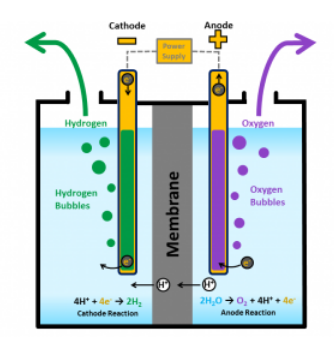
\includegraphics[width=0.5\linewidth]{figures/electrolysis.png}
	\hfill
	\caption{Production of hydrogen by electrolysis.}
	\label{fig:electro}
\end{figure}

\subsection{High-Temperature Electrolysis (HTE)}

Solid oxide electrolyzers must operate at thermperatures high enough for the solid oxide membranes to function properly (about 700$^{\circ}$-800$^{\circ}$C). The use of heat at these elevated temperatures decreases the amount of electrical energy needed to produce hydrogen from water. In the HTE process, nuclear thermal energy rather than electricity converts water to steam and then the electricity dissociates the water at the cathode to form hydrogen molecules \cite{xu_introduction_2017}.

\subsection{Iodine-Sulfur Thermochemical Cycle}

The concept of using nuclear heat and water allows the possibility of a sustainable production without greenhouse gases. The most simple and promising methods, in terms of efficiency, operate at very high temperatures, typically above 900$^{\circ}$C. For example, sulfur-based cycles (Fig. \ref{fig:isulfur}) use a sulfuric acid dissociation reaction that only works above 870$^{\circ}$C and whose efficiency increases with temperature \cite{cea_gas-cooled_2006}. The sulfur-iodine (SI) cycle results the best cycle for coupling to a high temperature reactor (HTR) due to its high efficiency. A General Atomics experiment has operated multiple times to produce hydrogen. The production was at a rate of 75 L/min. The same report estimates that a scaleup of the process using a 50 MWt Nuclear Reactor could produce 12000 kg/day of Hydrogen \cite{benjamin_russ_sulfur_2009}.
The Next Generation Nuclear Plant (NGNP) \cite{cea_gas-cooled_2006} aims to produce 500 kg/h of $H_2$ by using 50MWt.

\begin{figure}[H]
	\centering
	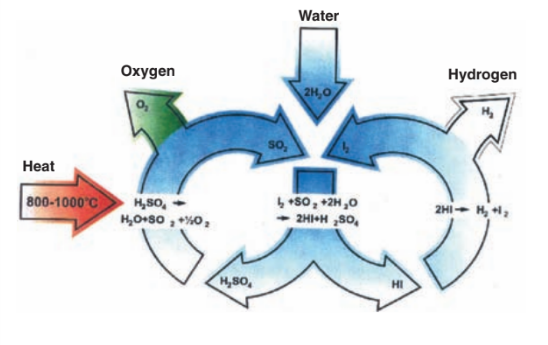
\includegraphics[width=0.5\linewidth]{figures/iodine-sulfur.png}
	\hfill
	\caption{Production of hydrogen by iodine-sulfur themochemical cycle.}
	\label{fig:isulfur}
\end{figure}

\section{Methodology}
\label{method}

A gasoline gallon equivalent (GGE) is the amount of fuel that has the same amount of energy as a gallon of gasoline. One kilogram of hydrogen is equivalent to one gallon of gasoline \cite{noauthor_hydrogen_nodate}. Burning a gallon of gasoline produces 19.64 lbs of CO$_2$ \cite{noauthor_how_2014}. 
Similarly, a diesel gallon equivalent (DGE) has the same amount of energy as a gallon of diesel. Approximately, a dge is 113\% of a GGE \cite{noauthor_fuel_2014}, then 1.13 Kg of hydrogen is equivalent to one gallon of diesel.
A gallon of diesel produces 22.38 lbs of CO$_2$ \cite{noauthor_how_2014}. 
Table \ref{tab:meth} summarizes this information.

\begin{table}[]
	\centering
    \caption{GGE, DGE, and CO$_2$ produced.}
    \label{tab:meth}
	\begin{tabular}{l|lll}
	\hline
	                 & Hydrogen & Gasoline    & Diesel      \\ \hline
	GGE              & 1 Kg     & 1 Gallon    & 0.88 Gallon \\
	DGE              & 1.13 Kg  & 1.13 Gallon & 1 Gallon    \\
    CO$_2$ produced  & -        & 19.64 lbs   & 22.38 lbs   \\ \hline

	\end{tabular}
\end{table}

\section{Results}

Figure \ref{fig:mtdfuel} shows the amount of diesel purchased every day by MTD in a year (how to cite this??/private communitcations). The calculations take into account the assumption that MTD consumed the purchased fuel on the same day.
Table \ref{tab:h2req} lists the required amounts of hydrogen to supply the MTD fleet. Average Gallons per day refers to the total amount of fuel consumed in a year averaged in 365 days.

\begin{figure}[]
	\centering
	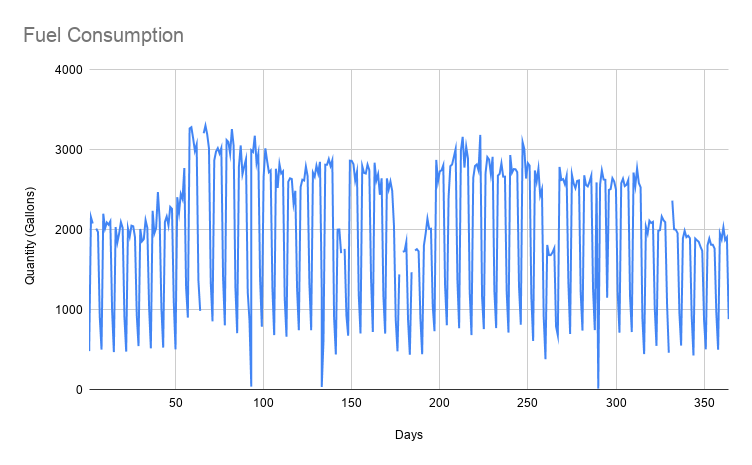
\includegraphics[width=0.6\linewidth]{figures/fuelconsumption.png}
	\hfill
	\caption{Quantity of gallons of diesel consumed each day by MTD from July 1st 2018 to June 30th 2019.}
	\label{fig:mtdfuel}
\end{figure}

For the case of the UIUC fleet, 227 passenger vehicles and 275 service vehicles compose the totality of the fleet \cite{noauthor_increase_2020}. The calculations consider only 108 vehicles chosen based on their annual mileage that consume 269 gasoline gallons per day \cite{holcomb_fueling_2015}. Table \ref{tab:h2req} lists the required amounts of hydrogen to supply the UIUC fleet.

\begin{table}[]
	\centering
    \caption{Hydrogen required and CO$_2$ produced by MTD and UIUC fleets.}
    \label{tab:h2req}
\begin{tabular}{l|rr}
\hline
                              & MTD (Diesel)     & UIUC (Gasoline)  \\ \hline
Average Gallons per day       & 1,971.8          & 269.0            \\
Kg of Hydrogen per day        & 2,228.2          & 269.0            \\
CO$_2$ Daily Emissions (lbs)  & 44,129.5         & 5,283.2          \\
Gallons per year              & 719,717.6        & 98,185.0         \\
Kg of Hydrogen per year       & 813,280.9        & 98,185.0         \\
CO$_2$ Yearly Emissions (lbs) & 16,107,279.9     & 1,928,353.4      \\ \hline
\end{tabular}
\end{table}

\section{Conclusion}

%%%%%%%%%%%%%%%%%%%%%%%%%%%%%%%%%%%%%%%%%%%%%%%%%%%%%%%%%%%%%%%%%%%%%%%%%%%%%%%%
\bibliographystyle{ans}
\bibliography{bibliography}
\end{document}

